\documentclass[11pt]{article}
\usepackage[margin=1.0in]{geometry}

\usepackage{wrapfig}
\usepackage{natbib}
\usepackage{graphicx}
\usepackage{hyperref}
\usepackage{float}
\usepackage{multirow}
\usepackage{siunitx}
\usepackage{bm}

\title{Novel Methods of Wavelength Calibration for Fiber-fed Radial Velocity Spectroscopy}

\author{Ryan Petersburg\\
Yale University Department of Physics\\
Advisor: Debra Fischer\\
\\
Thesis Prospectus}
\date{August 2018}

\begin{document}

\maketitle

\begin{abstract}

Measuring the radial velocity of a star to high precision hinges on the ability to accurately wavelength calibrate spectra.


Wavelength calibration is naturally a necessary step in spectroscopic measurement. Within the field of exoplanet detection through stellar radial velocities, however, extreme precision of wavelength calibration is absolutely critical. In the advent of Earth-like exoplanet discovery around G \& K spectral-type stars, the upper limit for these measurements is $10^{-11}$, or less than $10^{-4}$ \SI{}{\pico\meter} stability at \SI{1500}{\nano\meter}.

\end{abstract}

\pagebreak

\section{Introduction}

The discovery of less massive and longer period planets using the stellar radial velocity (RV) method requires an unprecedented level of spectroscopic precision. The current goal of RV spectroscopy is \SI{10}{\centi\meter\per\second} precision, a factor of 10 better than the current state-of-the-art spectrographs, thereby allowing the discovery of Earth-like planets orbiting G and K stars in their respective habitable zones \citep{Fischer2016}. The next-generation of visible-band RV spectrographs---including the EXtreme PREcision Spectrograph (EXPRES) \citep{Jurgenson2016}, the instrument most relevant to my research---are utilizing precision engineering and extreme environmental stability to reach this goal.

Regardless of the steps taken to stabilize the spectrograph, RV precision is ultimately limited by the ability to accurately calibrate stellar spectra. The process for wavelength calibration is rather intuitive: compare the absorption lines of the RV-shifted stellar spectrum with a well-known, un-shifted spectrum. There are three distinct steps to optimally achieve this goal:
\begin{enumerate}
    \item purchase or develop a calibration light source that fills the bandpass of the spectrograph while maintaining a level of stability within the RV precision requirements,
    \item optically couple the light source to the spectrograph detector without degrading the signal or introducing time-dependent shifts to the spectrum, and
    \item code an extraction algorithm that maximizes signal-to-noise and resolution of the calibration spectrum without increasing systematic error.
\end{enumerate}

For my thesis work, I am proposing novel methods that address each of these three steps. For simplicity, this prospectus (and my eventual dissertation) is organized into three major sections, each pertaining to my work with one of the above topics. Since these topics are so distinct, I provide background for them individually in each of the following sections, instead of trying to compact it all into the introduction. In Section \ref{sec:astrocomb}, I discuss my plans to develop a cheaper and more reliable wavelength calibration source by combining an electro-optic modulation comb with an aluminum nitride waveguide. In Section \ref{sec:modal_noise}, I present results from my previous work mitigating modal noise through optical fiber agitation and my plans to demonstrate how this work has improved EXPRES calibration. Finally, in Section \ref{sec:spec_perf}, I introduce Spectro-perfectionism and how I am developing a deconvolution algorithm to increase signal-to-noise and resolution for extracted wavelength calibration spectra.

\section{Aluminum Nitride Astrocomb \footnote{The work in this section was proposed to the NSF, NASA, and Keck Foundation, therefore much of the information here was drawn from those proposals.}}
\label{sec:astrocomb}

In order to extract stellar spectra, RV spectrographs use the spectra of well-characterized and stable light sources as a simultaneous reference on the spectrograph camera. Historically, thorium argon lamps and iodine reference cells have been used to calibrate RV spectrographs since their spectral properties are well understood and their bandwidth covers most of the visible spectrum. However, both of these light sources have inherent issues that limit RV measurements to approximately 1 m/s precision. Th-Ar emission lines are broad, saturated, and irregularly spaced, meaning some wavelength regions are less well calibrated than others. The iodine technique, which applies absorption wavelengths directly on the stellar spectrum, masks the subtle spectral line profile effects imprinted by stellar activity. Furthermore, iodine introduces complexity, such as parameter cross talk, to the forward modeling \citep{Spronck2015} and the cells themselves may not have long term mechanical stability \citep{Fischer2014a}.

More recently, RV spectrographs have employed frequency combs (FCs), synthesized spectra containing sharp peaks of intensity at equally spaced frequencies, with the intention of better stability and therefore precision in their wavelength calibration. Ideally, the lines of a FC are non-overlapping and located at precisely determined wavelengths with flat intensity, to avoid over- or under-saturating pixels on the spectrograph camera. The FC must also have the proper free spectral range (FSR, frequency separation of comb lines) across the entire bandwidth of the spectrograph optics so that the camera can resolve each peak (more than $\sim$\SI{10}{\giga\hertz}) and calibrate a sufficient number of stellar frequencies (less than $\sim$\SI{40}{\giga\hertz}). Also, the zero-point frequency offset ($f_0$) and FSR should not drift over both short (seconds) and long (months) time scales. Most FC devices have been developed for the near-infrared, due to the proliferation of telecom interest around \SI{1550}{\nano\meter}, and this has been sufficient for observing M dwarf exoplanets \citep{Fischer2016}. However, to address planetary system statistics for late F, G, and early K type stars, the wavelength range will need to stretch through the visible to better calibrate many more absorption lines. It is especially important to reach the Calcium H & K lines located below \SI{400}{\nano\meter} that contain chromospheric activity information which characterizes photospheric noise \citep{Isaacson2010, Lovis2011}.

A relatively cheap way to produce a broadband optical FC is using a tunable Fabry-Pérot (FP), a resonant cavity that employs feedback to correct for drifts in length. They do not offer an inherent $f_0$ calibration, however, and must be referenced against a separate stable source for bootstrapped calibration \citep{McCracken2014, Sturmer2017} meaning the system cannot be self-contained. Therefore, fixed-length FP etalons were developed to mitigate this issue. However, \citet{Reiners2014} and \citet{Wildi2012} have shown that the set distance between the two reflective surfaces still drifts unpredictably, especially over long time scales, thereby continuing to limit spectrograph precision to only ~1 m/s.

Menlo Systems has built perhaps the most advanced wavelength calibrator for visible RV spectroscopy, a laser FC that reaches $\sim$\SI{1}{\centi\meter\per\second} RV precision \citep{Probst2014}. This FC pulses a femtosecond mode-locked laser to produce high finesse lines and an extremely stable FSR. Unfortunately, these lines are too tightly spaced for RV spectrographs, therefore the system must use line-by-line spectral filtering with multiple tunable FP cavities to suppress most of the produced frequencies. There are consequently some critical limitations to this device: complexity, cost, and limited bandwidth. The Menlo FC requires a continuing service contract to properly maintain it and thus has not yet reach true ``turn-key'' status. Also, this technology costs approximately \$1,000,000, a prohibitive price point for smaller RV projects, and is extremely bulky, limiting its use to larger ground-based spectrographs. Furthermore, the system is still limited to \SI{$\sim$450}{\nano\meter} on the blue end thereby excluding the critical Calcium H \& K lines below \SI{400}{\nano\meter}.

Therefore, I am proposing to develop an affordable, compact, and direct-generation optical FC (or ``astrocomb'') that extends across the entire visible and near-infrared regimes from 350–\SI{2140}{\nano\meter}. This astrocomb will utilize two technologies that have been already been thoroughly developed:
\begin{enumerate}
    \item a near-infrared octave-spanning and self-referenced electro-optic modulation 10 GHz FC, and
    \item an aluminum nitride on-chip waveguide that uses nonlinear material properties to frequency double and triple the EOM FC.
\end{enumerate}
Upon completion, this technology will be immediately able to calibrate a wide range of RV spectrographs to $10^{-11}$ precision (corresponding to 1 cm/s RV on the EXPRES high resolution spectrograph for example) in the search for Earth-like exoplanets orbiting sun-like stars. This section begins with brief descriptions of the current advancement of both the EOM comb and AlN waveguides, followed by my planned contributions of applying these technologies to RV wavelength calibration.

Such a laser frequency comb has not yet been introduced to the RV community, therefore this aspect of the thesis would be a significant contribution.


\subsection{Background}

\subsubsection{Electro-optic modulation frequency comb}

The foundation of my proposed astrocomb is built upon a self-referenced cascading electro-optic modulation (EOM) comb that has already been developed at the National Institute of Standards and Technology (NIST) \citep{Cole2015, Beha2017, Carlson2017a}. The layout for this fully functional EOM system, described by \citep{Cole2015}, is shown in Figure 1a. This device feeds a \SI{1550}{\nano\meter} continuous wave pump laser through a series of electro-optic waveguides with sinusoidally varying voltages (precisely controlled by a \SI{10}{\giga\hertz} electronic oscillator) that add time dependent amplitude- and phase-shifts to the incident light. These modulators thereby split the pump laser into equally spaced (\SI{10}{\giga\hertz}) frequency sidebands with a combined bandwidth of approximately \SI{4}{\nano\meter} (Figure 1b). Then, the light is propagated through \SI{100}{\meter} of highly nonlinear fiber (HNLF), which broadens the spectral width to \SI{40}{\nano\meter} using self-phase modulation nonlinearity, and a FP filter cavity that suppresses high-offset electronic frequency noise (Figure 1c). A dispersion controller flattens the spectrum line-by-line and passes the pulses through an electro-optic gate that uses pulse selection to optionally decrease the FSR by integer factors. Finally, the light is amplified with an erbium doped fiber amplifier (EDFA) to \SI{2}{\watt} average power and propagated through \SI{8}{\meter} of HNLF, further broadening the comb to span the entire infrared octave between 1070 and \SI{2140}{\nano\meter} (Figure 1d).

NIST has shown that the $f_0$ of the EOM comb can be calibrated using f–-2f interferometry \citep{Beha2017}. Since the comb is octave-spanning, the 2140 nm line is frequency doubled and beat against the 1070 nm line. After this stabilization, the EOM comb was shown to have a fractional uncertainty of 3 x 10-13 at \SI{1}{\second} and 3 x 10-14 at \SI{1000}{\second} corresponding to $<$\SI{1}{\centi\meter\per\second} RV precision at both time scales \citep{Beha2017}. This technology is important to the astrocomb design because it was developed almost completely with commercial off-the-shelf products. Intensity and phase modulators, HNLFs, EDFAs, and FP filter cavities can be purchased relatively low-cost from many optics retailers. Also, \SI{10}{\giga\hertz} electronic oscillators can be locked to GPS and have inherent stability much higher than required by an astrocomb, meaning the FSR would not need to be externally controlled. Therefore, this EOM design could be replicated with little modification on any optics table.

[ADD CARLSON CITATION]

\subsubsection{Aluminum Nitride waveguide}

Optical nonlinearity is a strong tool that can be used on this near-infrared EOM comb to expand it into the visible spectrum. Second-order nonlinearities provide second harmonic generation (SHG), a specific form of sum frequency generation (SFG), that doubles the frequency of light incident on the nonlinear material (Figure 2b). Similarly, third-order nonlinearities provide third harmonic generation (THG) that triples the incident light frequency (Figure 2c). Silicon dioxide and silicon nitride, historically the most widely researched nonlinear waveguide materials, only have strong third-order nonlinearity. Aluminum nitride (AlN), on the other hand, is quickly gaining ground as a phenomenal material for on-chip nonlinear optics applications because it has both strong third-order and second-order nonlinearity as well as low loss over an extremely wide bandwidth from the ultraviolet to the mid-infrared \citep{Jung2016}. Therefore, AlN is ideally suited for application to a broadband astrocomb.

Also, AlN has the potential to produce a visible astrocomb through supercontinuum generation, without having to rely on SFG.

The Yale Nanodevices Laboratory (YNDL), led by Hong Tang, has developed a mature nanofabrication process for AlN that deposits the material with a predetermined geometry onto silicon nitride chips. Using this device, the YNDL has fabricated many on-chip AlN waveguides with varying lengths (\SI{300}{\micro\meter} to \SI{3}{\centi\meter} \citep{Xiong2012a}), thicknesses (330--\SI{1500}{\nano\meter} \citep{Pernice2012}), and shapes (e.g. differing radii of curvature). These tests also showed strong SHG in the AlN waveguides with differing wavelength-dependent throughput based on the associated geometries. More recently, the YNDL has explored more deeply into AlN microring resonators \citep{Jung2013, Guo2016}. For example, \citep{Jung2014a} demonstrated an AlN microring resonator that generated a green, red, and infrared FC using the Yale Exoplanet Laboratory (YEL) in-lab high-resolution spectrograph. The span of this comb is detailed in Figure 2. Although the microresonator FC is not stabilized as this proposal is drafted, it proves that sufficient power could be produced by the SHG and THG frequencies in AlN for detection by a RV spectrograph (with future research looking to stretch this to fourth harmonic generation).

Results from Hong's lab with 80 MHz source seem promising for this application.

\subsection{Optical and Electronic Design}

The EOM based FC will be combined with the AlN waveguide to produce a simplified astrocomb as shown in Figure 3. An EOM FC, spanning 1070 – 2140 nm, as shown previously in Figure 1, is produced with a 1550 nm pump laser. The FC is amplified by an EDFA and fed into an AlN waveguide that doubles and triples these frequencies producing a 20 GHz comb centered at 775 nm and a 30 GHz comb centered at 517 nm respectively. The FSR of the instrument is fixed by the GPS stabilized 10 GHz microwave oscillator, and the $f_0$ can be fixed to 3 x 10-11 fractional uncertainty using $f-2f$ feedback (from the EOM comb and AlN waveguide, respectively) to the pump laser. The spectrum is flattened through modification of the NIST EOM comb design and by careful consideration of the AlN waveguide geometry. The resultant 350 – 2140 nm FC is then used as a calibration source for an RV spectrograph (SPX) below 10 cm/s precision. Unlike the Menlo mode-locked laser comb that suppresses lines in its over-dense fundamental spectrum, this astrocomb will produce each line directly with minimal active filtering allowing for a plug-and-play approach to RV spectrograph calibration.

The first step will be to leverage NIST’s expertise in developing an octave-spanning EOM comb at the Yale Exoplanet Lab (YEL), the research group headed by this proposal’s PI Debra Fischer. I will seek to specifically eliminate the dispersion controller and reference FP cavities from the previous design. These devices require separate active monitoring adding undue complexity to the completed astrocomb. As explained by \citep{Beha2017}, the dispersion controller could be replaced by a passive SMF filter system to still get the same level of spectral flattening from the device and AlN SHG will replace the need for FP cavity references.

Upon completion of the EOM comb, I will characterize its spectral envelope and calculate the necessary flattening function. I will continue the YEL collaboration with the YNDL to explore possible AlN waveguide geometries that ideally flatten this EOM output spectrum to less than 10 dB variance (with a goal of 3 dB). This iterative process is relatively simple and cheap, since the fabrication device is well established and the raw materials are widely available. As part of this process, I will also characterize the throughput of the waveguide SHG and THG and observe how it applies to the expansion and flattening of the EOM comb.

Finally, I will design and fabricate the complete astrocomb at the YEL by optically combining the CW laser fed EOM FC and AlN waveguide with the proper amplification and alignment for sufficient spectral flattening and throughput. This process involves compacting the components into as little space as possible to allow for easy transport and application to a wide range of instruments. I also will extract the 1070 nm comb line produced by the EOM comb and beat it against the SHG 1070 nm line (frequency doubled from 2140 nm) produced by the AlN waveguide. Using this beat, I can then investigate methods using commercial products (such as proportional-integral-derivative controllers) to lock the $f_0$ set by the pump laser. Therefore, the astrocomb becomes completely self-referenced without the need for overly-complex monitoring equipment.

Feedback to temperature of pump laser to control central wavelength.

Feedback to microwave oscillator to control comb line spacing.

Feedback to modulator phase controllers to optimize width and initial comb.

\subsection{On-site Testing}

Subsequently, I will fully characterize the super continuum spectrum produced by the astrocomb using the Yale Doppler Diagnostic Facility, a high-resolution bench-mounted echelle spectrograph for prototype development located in the YEL clean room. Along with spectrum analyzers and associated electronics, I will show the astrocomb reaching a fractional uncertainty of less than 3x10-11 over short times scales. Finally, the astrocomb can be tested on-sky using EXPRES, an extreme precision RV spectrograph currently under construction by the YEL for the 4.2-meter Discovery Channel Telescope at Lowell Observatory and scheduled for commissioning in October 2017. EXPRES has a modular calibration light source design and will also be employing a Menlo mode-locked laser FC, therefore my astrocomb’s stability can be compared directly against the current standard in broadband wavelength calibration. The YEL also has access to the telescope for 70 nights per year, meaning that the astrocomb calibration precision of <10 cm/s can be demonstrated over many months of real-world use.

Can compare cross-correlations of Menlo LFC and astocomb to understand differences in precision.


\section{Modal Noise Mitigation \footnote{I have already written a paper on most of this topic, therefore much of this section is directly taken from \citet{Petersburg2018}}}
\label{sec:modal_noise}

Fiber coupling the spectrograph to the telescope has become an essential and standard method for planet hunting spectrographs. Separating the spectrograph from the telescope by a fiber tens of meters long enables the spectrograph to be located in a controlled environment, isolating it from vibrational and thermal noise. Linking the telescope to the spectrograph via fiber also leverages the spatial scrambling properties inherent to fibers that, for the most part, decouple input variations from the output producing a stable illumination of the spectrograph optics \citep{Hunter1992}. This effect has been amplified through the use of double scramblers \citep{Halverson2015a, Spronck2015} and non-circular fiber geometries \citep{Chazelas2010, Spronck2012, Plavchan2013}.

Optical fibers also transmit light from calibration sources, such as wavelength calibrators and broadband flat-field sources, to the spectrograph. Laser frequency combs, especially the  astrocomb \citep{Probst2014} recently deployed at HARPS and soon at EXPRES, produce thousands of ultra-narrow, evenly spaced emission lines over a wide frequency range. When these highly coherent lines propagate through a multi-mode fiber, they create a source of noise that limits the signal-to-noise ratio (S/N) of the instrument and potentially induces false RV signals in the data. This noise is caused by interference between the finite number of electromagnetic modes that can propagate along a multi-mode fiber, and therefore the term \textit{modal noise} has been coined for this effect \citep{Epworth1978}.

For this part of my thesis, I have discerned an optimal strategy for reducing modal noise using mechanical agitation on multi-mode fibers propagating coherent visible light. This section begins with a definition of modal noise and an exploration for how previous experiments have mitigated it through static and dynamic methods (Section \ref{subsec:modal_noise_intro}). I then describe a novel form of quasi-chaotic coupled agitation and discuss results that show improvement in S/N and RV precision (Section \ref{subsec:modal_noise_results}). Finally, I describe my efforts to build an optimal agitator for EXPRES and propose an experiment to approximate the improvements it makes to calibration spectra (Section \ref{subsec:modal_noise_testing}).

\subsection{Background}
\label{subsec:modal_noise_intro}

Light propagates through an optical fiber in an integer number of electromagnetic modes. The exact calculation for this value is nontrivial since it depends on the instantaneous fiber geometry, injection parameters, and many other variables. The maximum number of modes for a step-index circular cross-section fiber (propagating a relatively large number of modes) with a monochromatic light source is approximately
\begin{equation}
M_{circ} \approx \frac{4}{\pi ^2} V^2 = \frac{4}{\pi ^2} \Bigg( \frac{2 \pi r \mathrm{NA}}{\lambda} \Bigg) ^2.
\label{eq:max_modes}
\end{equation}
$V$ is the normalized frequency of the fiber rewritten in terms of $\mathrm{NA} = \sqrt{n_\mathrm{core}^2 - n_\mathrm{clad}^2}$, the numerical aperture of the fiber determined by the core ($n_\mathrm{core}$) and cladding ($n_\mathrm{clad}$) indices of refraction, the core radius $r$, and the wavelength $\lambda$ of propagated light. This approximation is more difficult for a rectangular fiber, but \citet{Nikitin2011} shows empirically using electromagnetic and geometrical arguments that
\begin{equation}
\frac{M_\mathrm{rect}}{M_\mathrm{circ}} \approx 2 \frac{ab}{\pi r^2}
\label{eq:prop_modes}
\end{equation}
where $a$ and $b$ are the side lengths of the rectangular cross-section. Notice that $ab$ and $\pi r^2$ give the areas for a rectangle and circle respectively. From this, we will assert more generally, with some rearrangement of Equation (\ref{eq:max_modes}), that
\begin{equation}
M_{s} \approx \frac{16}{\pi} C_{s} A \Bigg( \frac{\mathrm{NA}}{\lambda} \Bigg) ^2
\label{eq:mode_area}
\end{equation}
where $A$ is the cross-sectional area of the fiber and $C_{s}$ is a constant coefficient dependent on fiber cross-sectional shape such that $C_\mathrm{circ} = 1$ and $C_\mathrm{rect} = 2$. $C_{s}$ is so far unknown for more complicated geometries, but we assume that $C_{s} \sim 1$.

\begin{figure}
    \begin{center}
	    \includegraphics[width=0.5\textwidth]{images/fiber_example.pdf}
	\end{center}
	\caption{Examples of unmitigated modal noise for a \SI{200}{\micro\meter} circular (left), \SI{200}{\micro\meter} octagonal (middle), and \SI{100x300}{\micro\meter} rectangular (right) optical fiber. All three fibers shown here have approximately the same cross-sectional area, meaning that they each are propagating about the same number of electromagnetic modes (see Equation (\ref{eq:mode_area})). Brightness in this image is scaled by (photon count)$^{0.6}$ for better presentation of the range of speckle brightness. The contrast of the speckles is therefore \textit{worse} than what is shown here.}
\label{fig:fiber_example}
\end{figure}

When coherent light is propagated through a multi-mode fiber, a high contrast speckle pattern known as modal noise is produced at the output for both the near field (fiber face projected onto a detector, Figure \ref{fig:fiber_example}) and far field. Modal noise is an inherent property of all multi-mode fibers regardless of the cross-sectional core shape \citep{Sablowski2016}. It arises from light coupling from mode-to-mode as it propagates through the fiber, causing slight variances in the path length traveled and producing the observed interference pattern. For RV spectrographs, this causes two problems: (1) it limits the maximum S/N and (2) systematic variations in the speckle pattern will mask themselves as minute shifts on the focal plane causing errant RV signatures.

\subsubsection{Limit on S/N}

Due to its high contrast, modal noise can severely decrease the S/N of an RV spectrograph \citep{Epworth1978, Baudrand2001, Lemke2011, Iuzzolino2014}. For a fiber without spatial filtering or a slit, the magnitude of this noise is proportional to $\sqrt{M_s}$ \citep{Goodman1981}. Therefore, increasing the size of the fiber, increasing the numerical aperture of the fiber (or decreasing the injected focal ratio), and decreasing the wavelength of injected light should increase the S/N due to modal noise. It also appears that changing the fiber core shape could affect the S/N.

Experimental results of these conditions have been well documented. S/N due to modal noise has been shown empirically to
\begin{enumerate}
\item increase with larger fiber core cross-sectional area \citep{Lemke2010, Sablowski2016},
\item decrease with larger focal ratios \citep{Baudrand2001, Sablowski2016},
\item decrease with longer wavelength of injected light \citep{Baudrand2001},
\item slightly increase with more static bends in the fiber (changing the NA) \citep{Imai1979},
\item remain the same for differing fiber lengths greater than a few meters \citep{Baudrand2001}, and
\item improve for non-circular fibers over circular fibers \citep{Sablowski2016, Sturmer2016}.
\end{enumerate}
All of these results follow exactly from Equation (\ref{eq:mode_area}) and implies that fibers with non-circular geometries have larger $C_{s}$.

\subsubsection{Systematic variations}
\label{subsec:sys_var}

Since the resultant speckle pattern is dependent on dynamic optical properties of the fiber, modal noise can induce false RV's on the spectrograph \citep{Mahadevan2014}. The spectrograph input is directly imaged onto the detector, so any spatial variation in intensity of the injected light will change the apparent line spread function in the spectra and cause errors in the assigned RVs. If these drifts have some regular period, modal noise could even cause errant planet signatures.

As is clear in Equation (\ref{eq:mode_area}), modal noise is heavily wavelength dependent. When the center wavelength of a coherent light source changes, the speckle pattern subsequently shifts.  Speckle patterns can be visually distinguished when the injected wavelength of light changes by at least \SI{8}{\pico\meter} at \SI{1500}{\nano\meter} \citep{Redding2013}. Next-generation RV spectrographs are using laser frequency combs with $10^{-11}$ stability \citep{Probst2014}, or less than $10^{-4}$ \SI{}{\pico\meter} stability at \SI{1500}{\nano\meter}, rendering speckle drift due to wavelength drift effectively irrelevant. However, since the speckle pattern is smoothly wavelength dependent, the resultant spectral line spread function of a frequency comb is correlated between neighboring lines, meaning any drift due to modal noise is not necessarily randomly distributed across the spectrum.

The speckle pattern seen at the end of a fiber changes over time most commonly because of \citep{Epworth1978}:
\begin{enumerate}
\item temperature variation,
\item fiber input illumination variation, and
\item fiber movement (bending, twisting, etc.).
\end{enumerate}
These three conditions inevitably pose problems when imaging a spectrum since they are inherent to modern fiber-fed RV spectrographs \citep{Baudrand2001, Mahadevan2014}. There is typically a changing temperature differential between the telescope and the spectrograph, fluctuations in atmospheric density and guiding change the fiber illumination, and the telescope (along with the connected fibers) slowly moves throughout the night.

\subsubsection{Mitigation Techniques}
\label{subsec:mitigation}

\begin{table*}
\centering
\small
\caption{Previous Study of Dynamic Modal Noise Mitigation Methods}
	\small
	\begin{tabular}{llcc}
		\hline
		References & Method & Frequency & Amplitude \\
		\hline\hline
		\citet{Daino1980} & Loudspeaker & \SI{110}{\hertz} & ``Sufficient'' \\
		\hline
		\citet{Hill1980} & Turbulent Air Stream & ---- & --- \\
		\hline
		\citet{Baudrand2001} & --- & \SI{30}{\hertz} & \SI{1}{\milli\meter} \\
		\hline
		\multirow{2}{*}{\citet{Lemke2011}} & Loudspeaker & 1.5 Hz & --- \\
		 & Loudspeaker & \SI{80}{\hertz} & --- \\
		\hline
		\multirow{3}{*}{\citet{McCoy2012}} & Paint mixer & \SI{60}{\hertz} & --- \\
		 & Hand agitated & 1-\SI{2}{\hertz} & 10-\SI{15}{\centi\meter} \\
		 & Mechanical agitator & 2-\SI{3}{\hertz} & 1-\SI{5}{\centi\meter} \\
		\hline
		\multirow{2}{*}{\citet{Plavchan2013}} & ``Tweeter'' & \SI{100}{\hertz} & \SI{1}{\milli\meter} \\
		 & ``Woofer'' & \SI{1}{\hertz} & \SI{25}{\milli\meter} \\
		\hline
		\multirow{3}{*}{\citet{Mahadevan2014}} & Int. Sph. + Diff. & --- & ---\\
		 & McCoy agitator & 2-\SI{3}{\hertz} & 1-\SI{5}{\centi\meter} \\
		 & Hand agitation & 1-\SI{2}{\hertz} & \SI{10}{\centi\meter} \\
		\hline
		\multirow{2}{*}{\citet{Halverson2014}} & Int. Sph. + Diff. & --- & --- \\
		 & Int. Sph. + Rot. Mirror & --- & --- \\
		\hline		
		\citet{Roy2014} & Rail agitator & 1-\SI{2}{\hertz} & \SI{170}{\milli\meter} \\
		\hline
		\citet{Sablowski2016} & ``Rotating Excenter'' & \SI{2}{\hertz} & \SI{20}{\centi\meter} \\
		\hline
	\end{tabular}
\label{table:previous_studies}
\end{table*}

Modal noise can be mitigated by continuously exacerbating one of the above three dynamic variations, thereby shifting the speckle pattern throughout an appropriately long camera exposure and averaging out the noise. Controlled temperature variation (option 1) is non-ideal because a \SI{1}{\meter} fiber requires approximately $8 ^\circ \mathrm{C}$ amplitude fluctuations to visibly decorrelate the speckle pattern \citep{Redding2013}, and would be impractical to implement. Therefore, RV spectrographs have been left with either varying the illumination (option 2) or shaking the fiber (option 3). As summarized in Table \ref{table:previous_studies}, these modal noise reduction techniques have been discussed by many experiments concerned with RV spectroscopy.

\citet{Mahadevan2014} and \citet{Halverson2014} explore the effectiveness of varying the illumination on the fiber face. Using an integrating sphere, diffuser, and rotating mirror, they show gradual improvements in modal noise reduction due to the addition of further illumination variation. However, the integrating sphere, an integral part of these methods, has a throughput efficiency of approximately $10^{-6}$ and is not feasible to be introduced in the science light optical path. To allow flexible observing programs, particularly science observations bracketed by precision wavelength calibration sources, the modal noise mitigation technique needs to be more efficient.

Otherwise, the majority of these studies use various forms of agitation---including loudspeakers, paint mixers, and air streams---that shake the fiber over time. The variation in frequency and amplitude for these methods is unfortunately quite wide and conclusions are difficult to make. However, there have been slight trends in the results and the discussed assumptions so far are as follows:
\begin{enumerate}
\item The frequency of agitation should be greater than $1/\tau$, where $\tau$ is the exposure time \citep{Baudrand2001}.
\item Noise is more effectively reduced by high-amplitude motion \citep{Lemke2011, McCoy2012}.
\item More oscillations per exposure time (with an upper limit) provide further noise reduction \citep{Lemke2011}.
\item Combining a high-frequency ``tweeter'' with a high-amplitude ``woofer'' reduces noise effectively \citep{Plavchan2013}.
\item Hand agitation is better than any form of mechanical agitation \citep{Lemke2011, McCoy2012, Mahadevan2014, Roy2014}.
\item Non-harmonic or chaotic motion is recommended \citep{Grupp2003} though an exact method has not yet been experimentally tested.
\end{enumerate}
Although this has been good for subjective intuition, the exact mechanisms behind the improvements in S/N and prevention of RV drift due to fiber agitation have not yet been explored.

\subsection{Results from in-lab testing}
\label{subsec:modal_noise_results}

For this part my thesis, I have filled out the parameter space of fiber agitation methods further than previous studies. I am interested in seeing trends across different agitation amplitudes and frequencies, fiber shapes and sizes, and coupling permutations to make more precise conclusions about the nature of modal noise mitigation through fiber agitation. I present a few of the most important plots here, but details can be found in my publication on the subject \citep{Petersburg2018} and a full description of the experiment and my results will be included in my dissertation.

\subsubsection{Method of agitation and fiber geometry}

We compare the two individual agitation methods and coupled agitation using a collection of five fibers of varying shapes and sizes (see the legend in Figure \ref{fig:ag_snr}). The linear agitator is set to an amplitude of \SI{80}{\milli\meter} and the frequency of both agitators to \SI{1.0}{\hertz}. All images are taken with \SI{1.0}{\second} exposures.

Results for the single-rotation and 10-rotation cases are shown in Figure \ref{fig:ag_snr}. Across all fiber shapes and sizes and number of rotations, the linear agitator appears to be slightly better than the circular agitator. There is a similar increase in S/N when looking at coupled agitation in single-rotations. However, coupling the agitation over 10-rotations significantly increases the S/N for all fiber configurations.

\begin{figure}
\centering
	\includegraphics[width=0.5\columnwidth]{images/ag_snr.pdf}
	\caption{S/N comparison for varying fiber geometries and large-amplitude agitation methods. The S/N is presented for both single-rotation and 10-rotation images.}
\label{fig:ag_snr}
\end{figure}

To better understand why coupled agitation is more effective at reducing modal noise at longer exposures, we also analyze the effect of each agitation method over multiple rotations, as shown in Figure \ref{fig:rect_snr_vs_time} for the \SI{100x300}{\micro\meter} rectangular fiber. The S/N shows significant improvement beyond a single rotation when coupling the agitation methods. The rate of this improvement is about the same (if not slightly better) than that when the fiber is lit by an LED, a relatively incoherent source. Circular and linear agitation, on the other hand, effectively plateau after the first rotation. We see identical effects for all of the remaining fiber shapes and sizes.

\begin{figure}
\centering
	\includegraphics[width=0.5\columnwidth]{images/rect_snr_vs_time.pdf}
	\caption{S/N dependence on number of rotations for the \SI{100x300}{\micro\meter} rectangular fiber using various agitation methods. We find similar relationships for the all of the remaining fiber shapes and sizes.}
\label{fig:rect_snr_vs_time}
\end{figure}

10-rotation images of the three larger fibers using the coupled agitation method are shown in Figure \ref{fig:fiber_improved}. Compared to those shown in Figure \ref{fig:fiber_example}, the speckle patterns that appear when using coupled agitation are nearly nonexistent.

\begin{figure}
    \begin{center}
    	\includegraphics[width=0.48\textwidth]{images/fiber_improved.pdf}
    \end{center}
	\caption{10-rotation, coupled agitation images using the same three fibers shown in Figure \ref{fig:fiber_example}.  The diffraction pattern is clearly seen, but otherwise, the presence of speckles in these images is significantly diminished. Brightness is directly scaled with photon count in these images.}
\label{fig:fiber_improved}
\end{figure}

\subsubsection{Amplitude and frequency of agitation}

We use the \SI{100x300}{\micro\meter} rectangular fiber and the two agitators separately to test the effects of agitation amplitude and frequency of rotation on the S/N. We can only test amplitude on the linear agitator and take an image set for each position on the rotating arm. We test frequency on each of the linear and circular agitators at approximately equally spaced frequencies across their entire frequency range.

Results from these tests are shown in Figure \ref{fig:amp_freq_snr}. There is a strong positive correlation between linear agitation amplitude using both the single-rotation and 10-rotation analyses. There also appears to be a slight increase in S/N for the linear agitator at higher frequencies after ten rotations; however, there is no such increase for the single-rotations or any of the frequencies when using the circular agitator.

\begin{figure}
\centering
	\includegraphics[width=\textwidth]{images/amp_freq_snr.pdf}
	\caption{S/N comparison for varying amplitudes using the linear agitator (left) and varying frequencies using each of the linear (center) and circular (right) agitators.}
\label{fig:amp_freq_snr}
\end{figure}

\subsubsection{RV precision}

As discussed in Section \ref{subsec:sys_var}, optical fiber modal noise is an issue of centroid drift as well as diminished S/N. To observe how the centroid actually drifts over time, we test our agitation method on the \SI{100x300}{\micro\meter} rectangular fiber over three hundred \SI{1.0}{\second} exposures.

The resultant RV precision ($\sigma_{RV}$) due to a shifting speckle pattern centroid at the end of a fiber is calculated as
\begin{equation}
\sigma_{RV} \approx \frac{c}{R} \frac{\sigma_d}{D},
\label{eq:rv_error}
\end{equation}
where $c$ is the speed of light in a vacuum, $R$ is the resolution of the spectrograph, $\sigma_d$ is the standard deviation of fiber near-field centroid drift in the dispersion direction, and $D$ is the slit width (or short-end length of a rectangular fiber). Please see \citet{Petersburg2018} for a full derviation. Notice that for a $R=150,000$ spectrograph fed by a \SI{33}{\micro\meter} slit attempting to reach \SI{1.0}{\meter\per\second} RV precision per line, the required stability of the centroid along the dispersion direction is \SI{0.0165}{\micro\meter}.

Importantly, $\sigma_{RV}$ is only the RV error \textit{per resolution element} or \textit{per line} from a wavelength calibration source. Averaging over $N$ lines with independent modal structure, we can divide $\sigma_{RV}$ by $\sqrt{N}$ to approximate total RV error. $N$ may not necessarily equal the total number calibration lines, however, since two neighboring wavelengths may propagate with the same number of modes and thus the same modal structure. Recall from Equation (\ref{eq:mode_area}) that the number of supported modes is a function of wavelength. With a high number (thousands) of propagating modes, we do not expect adding or subtracting a single mode will result in a statistically independent modal noise structure. Though, such a study is beyond the scope of this paper.

However, assuming a difference in 10 supported modes makes the structure effectively independent, we assert
\begin{equation}
N \approx \frac{M_s(\lambda_{min}) - M_s(\lambda_{max})}{10},
\label{eq:N}
\end{equation}
where $\lambda_{min}$ and $\lambda_{max}$ are, respectively, the minimum and maximum wavelengths of the relevant calibration region. Note that the calibration source needs to be sufficiently dense (i.e. the number of lines is greater than $N$) to properly use this approximation. Even though Equation (\ref{eq:N}) has not been empirically tested, since it requires a comprehensive study on the systematic correlation of modal noise, we believe it to be a rather conservative estimate for statistical reduction.

The idealized agitation method we use to test RV precision includes the circular agitator oscillating at \SI{1.1}{\hertz} and the linear agitator set at \SI{240}{\milli\meter} and \SI{1.0}{\hertz}. Keeping the two agitators at slightly different frequencies means that phase between them constantly changes and a large range of fiber configurations are reached after about \SI{10}{\second}.

We compare this idealized method to the LED source (low modal noise), a slowly agitated fiber (high modal noise), and a fiber moved as if it were attached to a telescope (very high modal noise). For the slow agitation test, we set only the linear agitator at \SI{80}{\milli\meter} and \SI{0.03}{\hertz} meant to simulate a worst-case simple harmonic agitation method. To simulate the telescope motions, we use the linear agitator with \SI{80}{\milli\meter} amplitude but do not rotate continuously. Rather, we leave the agitator off most of the time except to turn it on briefly (about a quarter or half rotation) every 50 images. This approximates two conditions of the telescope: nearly still while tracking a star and sudden motion while switching targets.

To calculate the RV error, we first find the centroid within the fiber face for each image, relative to the center of the fiber in order to remove the observable ($\sim 2$ pixel) drift of the fiber stage. We then project this centroid drift along the short axis of the rectangle. We also average these centroids over sets of 10 and 30 images to approximate the centroid drift for longer exposure times. For each length of exposure, we calculate the standard deviation of the centroid drift and convert all values to RV using Equation (\ref{eq:rv_error}). The dispersion direction for a rectangular fiber is along the short end, meaning that the slit width $D$ is \SI{100}{\micro\meter}. The resolution of EXPRES is 150,000 for a \SI{33x132}{\micro\meter} rectangular fiber, so we use $R=50,000$ in Equation (\ref{eq:rv_error}) since our test fiber is three times as wide as the EXPRES fiber in the dispersion direction.

\begin{figure}
\centering
	\includegraphics[width=\textwidth]{images/rv_error.pdf}
	\caption{Centroid drift and resultant RV error for a fiber moved by a simulated telescope (first), slowly agitated fiber (second), coupled agitated fiber (third), and LED illumination (fourth). Each line represents a different exposure time each with their own calculated RV error. Note that the scale for the top three plots are different.}
\label{fig:rv_error}
\end{figure}

The results, shown in Figure \ref{fig:rv_error}, indicate that continuous agitation is essential to control modal noise. The simulated telescope yields RV errors above \SI{20}{\meter\per\second} that do not average out well with longer exposures. Using our idealized method of coupled agitation reduces errors from slow agitation by about 5--8 times and are so far minimized to about \SI{60}{\centi\meter\per\second} when using \SI{30}{\second} exposures. The minimum RV error we could measure in this test, by using the LED source, was \SI{26}{\centi\meter\per\second}. Therefore, our coupled agitation method is less than a factor of 3 from reaching our noise floor.

The calculated \SI{60}{\centi\meter\per\second} error for coupled agitation is the RV error \textit{per line} in the spectrograph. Thus, the total RV error could be reduced to below \SI{10}{\centi\meter\per\second} with only 36 mode-independent calibration lines. EXPRES is using a laser frequency comb with approximately {\SI{14}{\giga\hertz}} line spacing across 450-{\SI{700}{\nano\meter}} fed by a {\SI{33x132}{\micro\meter}} rectangular fiber at $f/3.0$ resulting in almost 17,000 calibration lines. Applying Equation (\ref{eq:N}), EXPRES will have $N=350$, reducing the expected RV error of the instrument to less than {\SI{3.2}{\centi\meter\per\second}}.

\subsection{EXPRES agitator and proposed testing}
\label{subsec:modal_noise_testing}

\begin{figure}
    \centering
    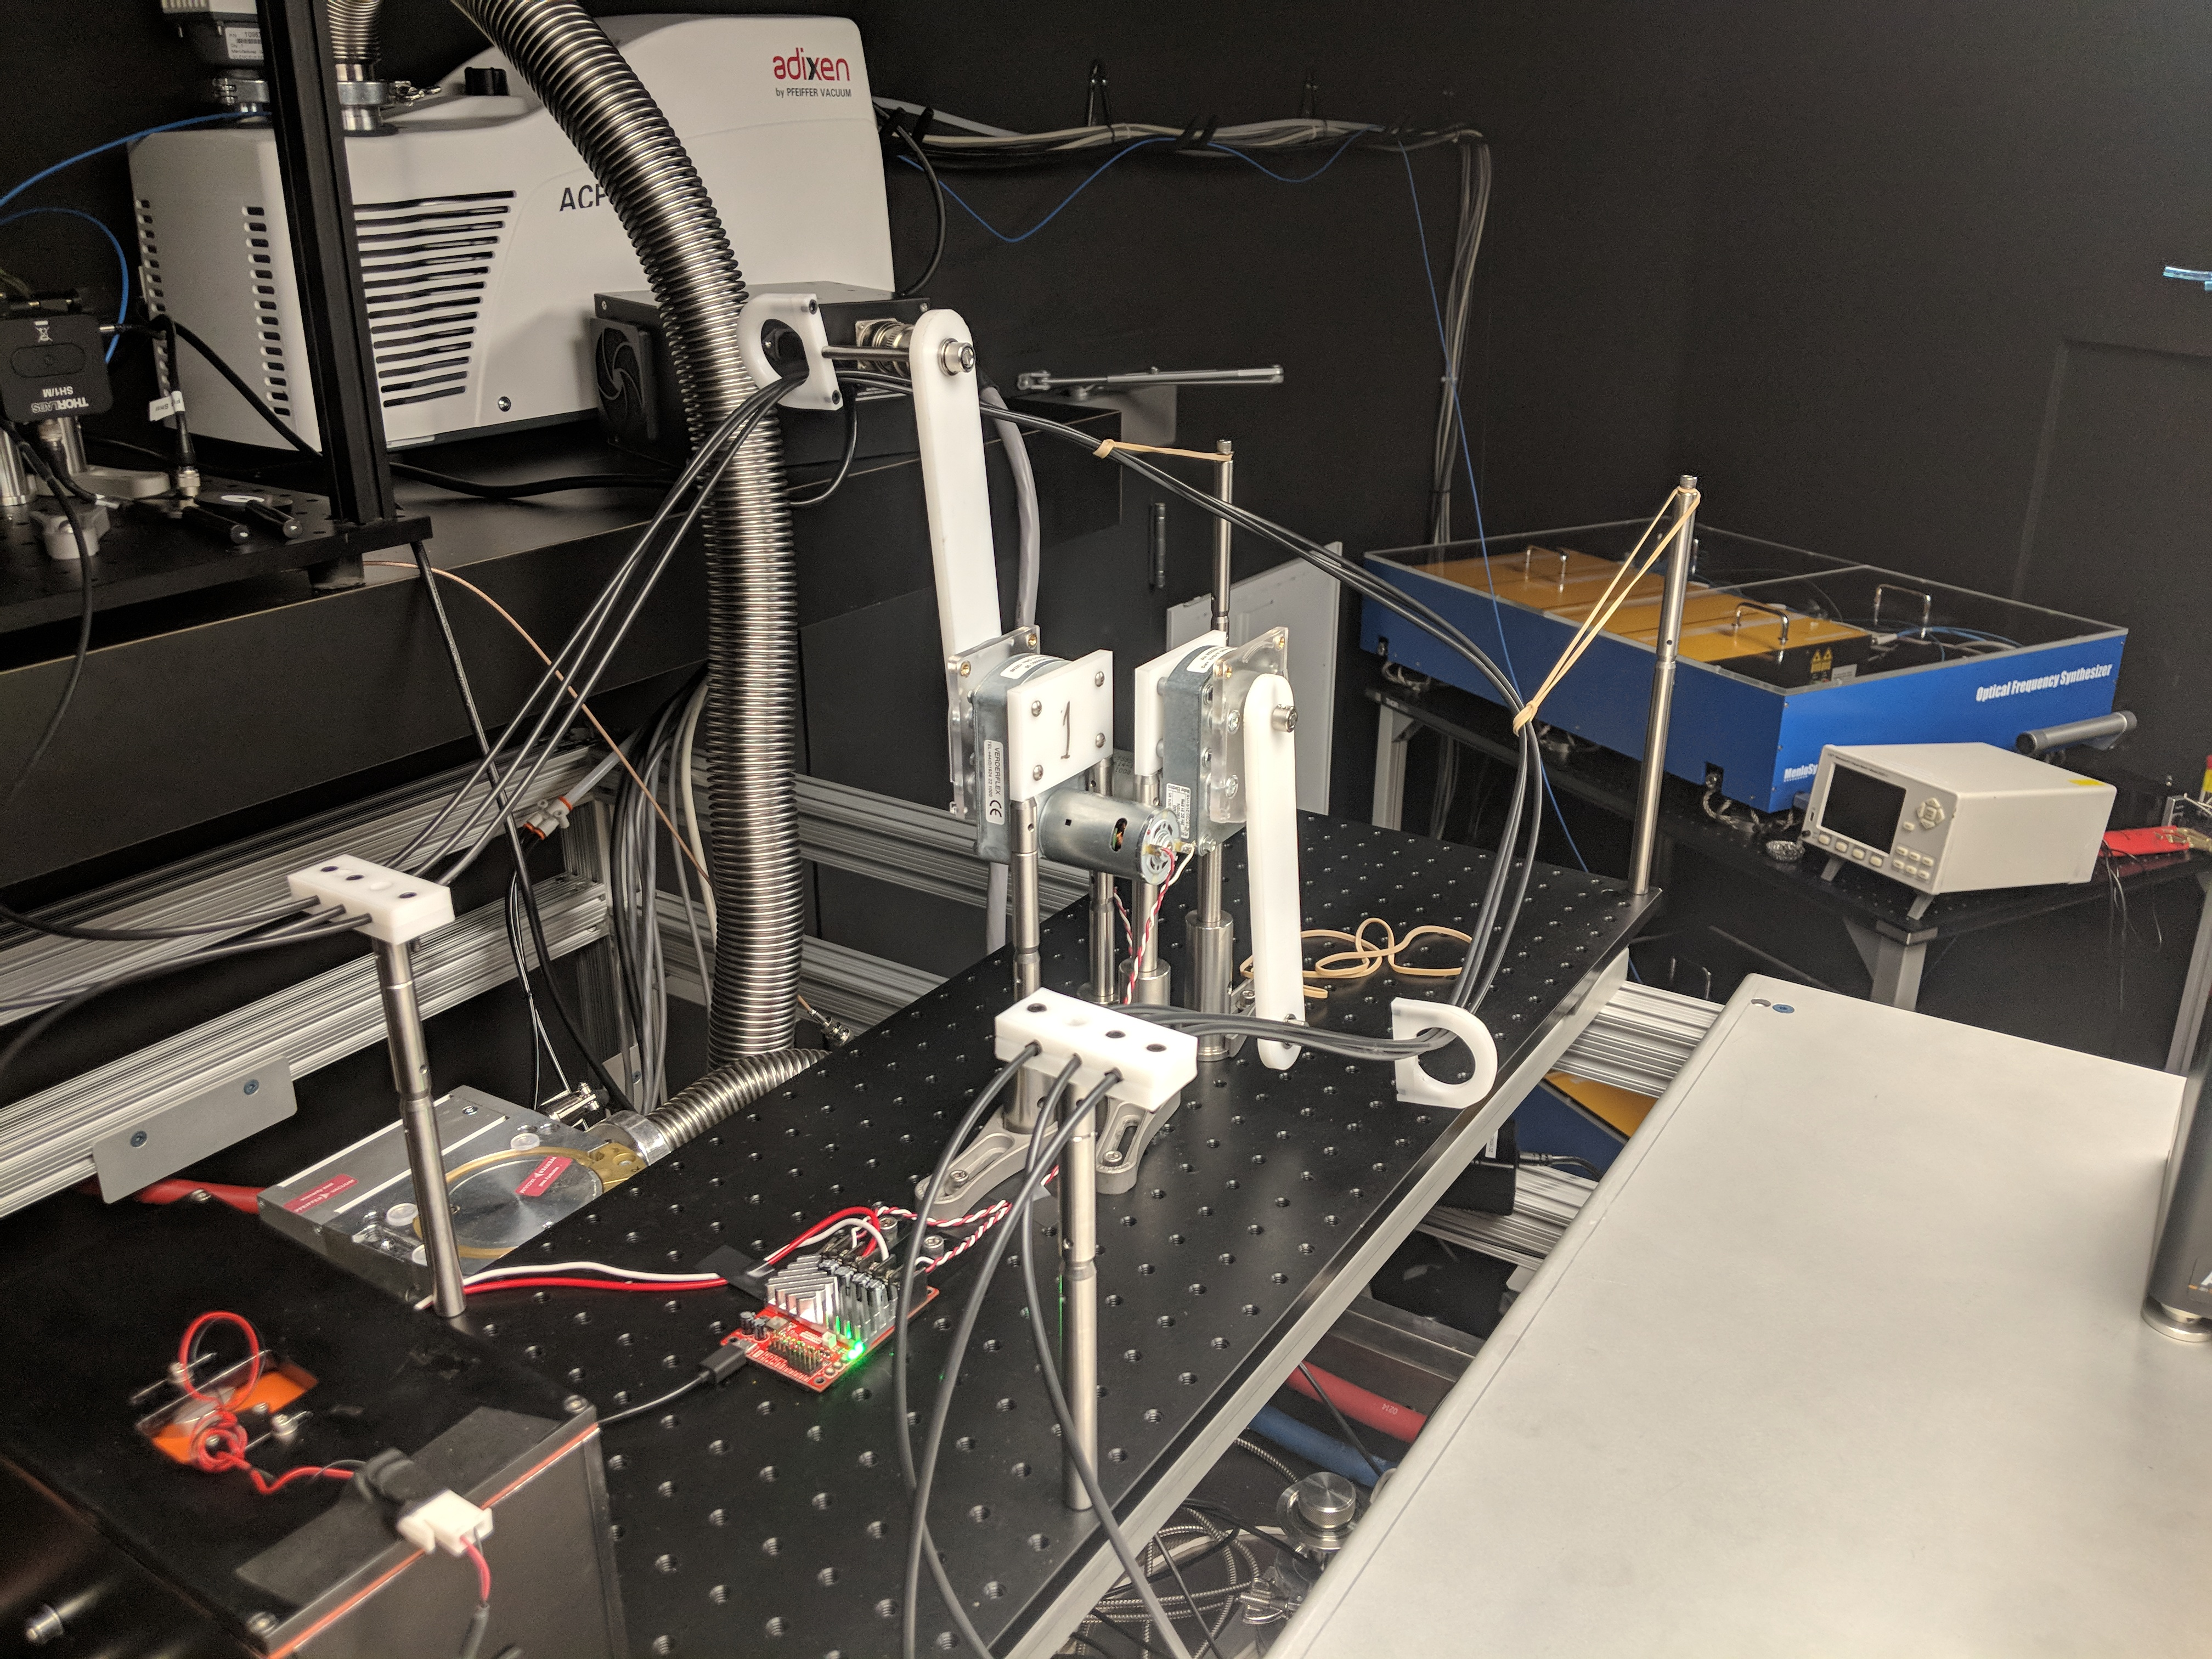
\includegraphics[width=0.75\textwidth]{images/agitator.jpg}
    \caption{Picture of the agitator installed with EXPRES at the Discovery Channel Telescope. The fiber is restrained by rubber bands in this image, but a recent update replaced those with longer-lasting springs.}
    \label{fig:agitator}
\end{figure}

These data were used to influence an agitator that I designed, built, and installed with EXPRES. As shown in Figure \ref{fig:agitator}, the agitator has two arms that each rotate independently using separate voltage-controlled DC motors. I have set these arms to rotate at \SI{0.45}{\hertz} and \SI{0.5}{\hertz} for every exposure, including wavelength calibration, flat-fielding, and stellar observations. These frequencies were chosen to maximally change the phase between the two arms within every exposure without over-stressing the fibers. That being said, the agitator has been in use since the beginning of 2018 and there has yet to be any sign of fiber degradation caused by agitation.

Now that this fiber agitator is installed on an active spectrograph, I would like to study the effects and mitigation of modal noise on a series of wavelength calibration spectra as the final step in this section of my thesis. There are two fundamental questions I would like to answer:
\begin{enumerate}
    \item To what extent does fiber agitation improve errors to the wavelength solution caused by modal noise and does this improvement follow the same trend as seen in the above results?
    \item Does modal noise introduce correlated errors in the spectrograph wavelength solution or is it effectively random?
\end{enumerate}
The data for this experiment will be EXPRES wavelength calibration spectra (ThAr and Menlo LFC) with the agitator turned on and off. I will also vary the length of exposures (after changing the intensity of each light source using neutral density) for both of these cases in a similar way to the above experiments. By comparing the wavelength solutions extracted from these sets of data, I will be able to answer the above questions respectively:
\begin{enumerate}
    \item If the scatter in residuals of the wavelength solution decrease with longer exposure time (i.e. more agitation), then there would be evidence that agitation is worthwhile for RV spectroscopy.
    \item Assuming errors when the agitator is turned on are randomly distributed, if there is a trend to the difference between the wavelength solutions when the fiber agitator is on or off (i.e. the difference in one line strongly predicts the difference in the neighboring line), then there is evidence that modal noise is correlated by wavelength.
\end{enumerate}
I expect to be able to complete these tasks with about a month of work, once the Menlo LFC comes back online and the EXPRES group develops a standardized method of calculating the wavelength solution.

\section{Spectro-perfectionism}
\label{sec:spec_perf}

With a high precision light source and a low noise optical coupling scheme, all that is necessary is a reliable way to convert the two-dimensional echellogram of the wavelength calibration source into a one-dimensional spectrum. This process is called \textit{extraction} and there are a myriad of methods that can accomplish this goal. Optimally, an extraction algorithm would maximize resolution and signal-to-noise of the data without altering the spatial positions of the calibration lines. Because, after extraction, a wavelength calibration spectrum should yield a wavelength solution that accurately corresponds each pixel of an extracted stellar spectrum to a wavelength, thereby enabling precise RV measurement.

Therefore, for the final part of my thesis, I am developing an extraction algorithm that uses the instrument's point spread function (PSF) to ``perfectly'' extract spectra. This algorithm, coined ``spectro-perfectionism'' by \citet{Bolton2009}, is meant to compete with the current standard in RV data processing, ``optimal extraction'' \citep{Horne1986}. In this section, I briefly describe the history of optimal extraction and spectroperfectionism before introducing my revised methods (Section \ref{subsec:spec_perf_intro}). Then, I describe the need for accurate point spread function modelling and detail my past efforts into doing so for EXPRES (Section \ref{subsec:psf}). Finally, I lay out some preliminary results using this data and how I intend to compare my algorithm directly against optimal extraction.

\subsection{Background \footnote{The introductory information in this section is primarily a distillation of the descriptions from \citet{Zechmeister2013} and \citet{Bolton2009}}}
\label{subsec:spec_perf_intro}

In principle, fiber-fed echelle spectrograph extraction is a discrete convolution problem. The (bias, dark, and background subtracted) CCD data ($D_{x,y}$) with pixel indices $(x, y)$ is a convolution of the spectral intensities ($s_\gamma$ at wavelength $\gamma$) and the instrument's wavelength-dependent PSF ($\Psi_{x,y,\gamma}$) with added noise ($n_{x,y}$):
\begin{equation}
    D_{x,y} = \sum_\gamma \Psi_{x,y,\gamma} s_\gamma + n_{x,y}.
\label{eq:convolution}
\end{equation}
With this in mind, and assuming that the noise if approximately gaussian, extraction is therefore ``simply'' a linear least-squares problem
\begin{equation}
    \chi^2 \approx \sum_{x,y} w_{x,y} \bigg[D_{x,y} - \sum_\gamma \Psi_{x,y,\gamma} s_\gamma \bigg]^2
    \label{eq:least_squares}
\end{equation}
where $\chi^2$ must be minimized. The weights $w_{x,y}$ are typically determined using a noise model $\sigma_{x,y}$ and a binary mask $M_{x,y}$ (removing bad pixels and pixels outside each echelle order) such that $w_{x,y}=\frac{M_{x,y}}{\sigma^2_{x,y}}$. In this section, I will be addressing two methods that can be used to solve Eq. \ref{eq:least_squares}: (1) optimal extraction and (2) spectro-perfectionism.

The current standard of fiber spectrograph extraction is the optimal technique, originally devised by \citet{Horne1986} but later refined in multiple papers, including (but not limited to) \citet{Piskunov2002} and \citet{Zechmeister2013}. This method makes the assumption that the PSF is a 1D slit function, thereby associating each column of an echelle order to a wavelength ($\gamma \rightarrow x$). Thus, the PSF can be rewritten in terms of a Kronecker delta
\begin{equation}
    \Psi_{x,y,\gamma} = \delta_{x,\gamma}\psi_{\gamma,y}
\label{eq:psf_optimal}
\end{equation}
and Eq. \ref{eq:convolution} simplifies to
\begin{equation}
    D_{x,y} = \psi_{x,y} s_x + n_{x,y}.
\end{equation}
Now, Eq. \ref{eq:least_squares} is solvable (setting $\frac{\partial}{\partial s_x} \chi^2 = 0$) for all $x$
\begin{equation}
    s_x = \frac{\sum_y w_{x,y} \psi_{x,y} D_{x,y}}{\sum_y w_{x,y} \psi^2_{x,y}}.
\end{equation}
The only thing remaining is to determine $\psi_{x,y}$. There are two possible approaches:
\begin{enumerate}
    \item make an initial guess (probably using $D_{x,y}$) and then iterate between extracting the spectrum and constructing a new $\psi_{x,y}$ based on the result \citep{Horne1986, Piskunov2002}, or
    \item use a low noise flat-field image $F_{x,y}$ that is taken by feeding a flat light source through the same path as the stellar spectrum. This image can be normalized (and possibly fit) to approximate $\psi_{x,y}$, or it can be used without normalization to produce a flat-normalized spectrum \citep{Zechmeister2013}.
\end{enumerate}

Although this method of optimal extraction has proven to be extremely prolific in the field of radial velocity echelle spectroscopy, it has a significant flaw: it does not take into account the full 2D PSF of the instrument. Thus, optimal extraction assumes that the spectrograph slit is uniformly aligned to the columns of the CCD and that the spectral information of a single wavelength bin is entirely contained in that column. However, the point spread function of echelle spectrographs typically envelope multiple columns of pixels (EXPRES was designed for a resolution element with 4 columns) and slight alignment errors could add an angle to the slit function (not even taking into account the possibility of a varying slit function angle across the CCD).

Therefore, \citet{Bolton2009} rather found a solution to Eq. \ref{eq:least_squares} directly without any assumptions while using the entire 2D PSF. This solution in matrix notation is
\begin{equation}
    \textbf{s} = (\bm{\Psi}^T \bm{N}^{-1} \bm{\Psi})^{-1} \bm{\Psi}^T \bm{N}^{-1} \bm{D}
    \label{eq:bolton_solution}
\end{equation}
where $\bm{N}$ is the pixel noise matrix. Since pixel errors are typically treated as independent, this matrix tends to be diagonal.

As explained by \citet{Bolton2009}, Eq. \ref{eq:bolton_solution} is actually a deconvolution algorithm. Since this algorithm yields a solution that exceeds the physical resolution of the instrument, it introduces severe ringing to the ultimate spectrum. However, this can be solved by reconvolving the spectrum back to the expected resolution.

\citet{Bolton2009} have demonstrated that this technique yields better signal-to-noise than optimal extraction. However, they were only able to show this using simulated data that was, at most $51\times101$ pixels in size. Therefore, I am interested in expanding their work through a few different avenues.
\begin{enumerate}
    \item Since the \citet{Bolton2009} data is purely simulated, they knew the exact PSF before executing the alorithm. I would need to measure the pixel-dependent PSF of EXPRES to even begin to use spectro-perfectionism.
    \item The EXPRES spectrograph CCD is $10k \times 10k$ pixels, much larger than the simulated data in \citet{Bolton2009}. Eq. \ref{eq:bolton_solution} is computationally expensive since the matrix $\Psi$ requires a PSF model for every wavelength bin.
    \item Eq. \ref{eq:bolton_solution} is a deconvolution algorithm, meaning it yields a solution that exceeds the physical resolution of the instrument. This introduces severe ringing to the resultant spectrum. \citet{Bolton2009} found a solution that involves ``reconvolving'' the spectrum back to the expected resolution, but this relies on taking the matrix square root of $\bm{\Psi}^T \bm{N}^{-1} \bm{\Psi}$ which is even more computationally expensive than the initial deconvolution.
\end{enumerate}
In the following sections, I detail my efforts to solve each of these problems and my expected results for my thesis.

\subsection{Point Spread Function Modeling}
\label{subsec:psf}

The first step in constructing a spectro-perfectionism algorithm is determining the PSF of the instrument. Typically, the PSF of an instrument might be constant across the entire CCD, allowing simplification of the deconvolution. However, the PSF of EXPRES changes significantly between orders and even slightly along a single order. For example, the height of each order is about two pixels larger for the bluest orders when compared to the reddest orders.

Therefore, a parameterized 

Need an accurate representation of the PSF parameters across the entire CCD.

Convolving a rectangle with a Gaussian makes a lot of sense intuitively for the spectrograph optics.

Also good because it means we could easily craft a deconvolved PSF if we wanted.

Sparse emission sources are good for this. ThAr is not ideal because there are many doublets and background continuua that make things complicated. Microcomb might not be ideal due to improper stability of the pump laser. These values were stable to only about 1pm, which is visible to the spectrograph on the order of 1/2 a pixel.

\subsection{Improving the spectro-perfectionism algorithm}

Going with Regularized Gold Deconvolution to prevent undersampling from the resultant image.

Apparent increase in LFC resolution and S/N without changing the fidelity of the stellar spectra.

Use 51Peg to compare RV results. It will be good to see the scatter and errors from expected RV results.

\section{Discussion and Proposed Timeline}

Finishing up with modal noise work. Already have published paper from this (Feb 2018). Can take EXPRES data by end of year (once engineering improvements are made).

Spectro-perfectionism is a work in progress. Hoping to draft a paper by the end of the year, with potential results from 51 Peg by then.

Astrocomb is a very long-term goal that might not even be finished by the time I graduate. I am hoping to complete a prototype of the un-stabilized version, but a complete build would probably need to be picked up by a postdoc once I am gone.



\pagebreak

\bibliographystyle{aasjournal}
\bibliography{thesis_prospectus}

\end{document}